\RequirePackage[l2tabu, orthodox]{nag}
\documentclass[12pt]{scrartcl}

\usepackage{amssymb,amsmath,verbatim,graphicx,microtype,upquote,units,booktabs,siunitx,xcolor,textcomp,tikz,gantt,coloremoji,graphics,hyperref}

\title{Bae Watch}
\subtitle{Fake Tinder For Fake Relationships}
\date{March 1\textsuperscript{st}, 2017}
\author{Illya Starikov}

\newcounter{tasks}
\setcounter{tasks}{0}
\newcommand{\task}[1]{%
    \addtocounter{tasks}{1}
    \subsubsection*{Task \#\thetasks: #1}
}

\newcommand{\shellcmd}[1]{\texttt{\colorbox{gray!30}{\strut#1}}}

\begin{document}
\maketitle

There is a growing problem in America: millennials. Millennials are subjectively proven to be the laziest, financially illiterate, entitled, and downright spoiled generation. The most disturbing thing about the millennial generation: their inability to get married before the age of \num{21}. This not only poses a problem with family, but friends as well. At any social gathering, whether it be dinner with friends, thanksgiving, or even the bar with friends, relationship questions for singles are unavoidable. Questions like the following can be expected: 

\begin{itemize}
    \item ``Isn't it time to settle down and find yourself a significant other?''
    \item ``Ayo when you gunna bring round a girl like the last one, she was 🔥🔥''
    \item or ``When are you going to find a good, Christian girl?''
\end{itemize}

\noindent A possible solution? Bae Watch.

\section{Objectives}
The objective of Bae Watch is simple: find an idealized relationship to ward off unsavory family members and friends. This is accomplished by leveraging the power of social networking. Users submit required information, which is mostly scraped off Facebook, and begin filtering through potential candidates. They do so through a swipe left for ``like'' and right for ``oh hell no''. It is a Tinder-esque (Figure~\ref{fig:tinder}) mechanic, but there's is something unique that Bae Watch brings: the kinds of data it requires.

\begin{figure}[!ht]
    \centering
    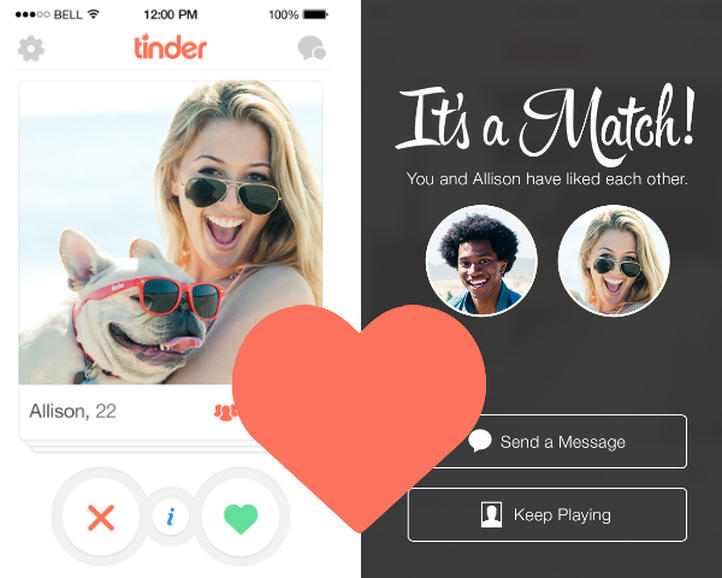
\includegraphics[width=.6\textwidth]{tinder}
    \caption{The real Tinder.}\label{fig:tinder}
\end{figure}

Besides the basic information that Facebook asks for (date of birth, favorite movies, IP addresses, all previous browsing history, etc.), we request information about the company you are trying impress. Things could include:

\begin{itemize}
    \item Religious preferences.
    \item Minimal salary.
    \item Preferred level of education (i.e. Bachelors, Masters, Doctor of Philosophy) and graduating major.
\end{itemize}

And other similar data. After aggregating said data, Bae Watch's AI\footnote{A bunch of \shellcmd{if} statements.}, Machine Learning\footnote{More \shellcmd{if} statements.}, and Algorithms\footnote{You guessed it. \shellcmd{try} and \shellcmd{catch} blocks.} present the user with the most likely matches. The foremost will be the most likely to impress, and subsequent users will more likely be English majors.

\section{Work Plan}
The week will begin on the second week of school, and prolong to the end of the semester. As any large scale engineering project, there will be a design phase --- specifically, wireframes for the User Interface and a Server Specifications will be made. Upon completing said specifications are made, the majority of the process will be put into creating the server and client. Both the server and client will be available as private (separate) repositories on \href{https://github.com}{Github} to monitor progress, commits, documentation, etc.

This can be eloquently described by the following Gantt chart.

\resizebox{\columnwidth}{!}{%
\begin{gantt}{17}{16}
    \begin{ganttitle}
    \numtitle{2}{1}{17}{1}
    \end{ganttitle}
    \ganttbar[color=red]{Design Server Specification}{0}{1}
    \ganttbarcon[color=red]{Write MVP Server}{1}{4}
    \ganttbarcon[color=red]{Write Full Server}{5}{6}
    \ganttmilestonecon[color=red]{Server Finished}{11}
    \ganttcon{11}{4}{11}{10} % Server Finished -> Integration

    \ganttbar[color=blue]{Wireframe Client}{0}{2}
    \ganttbarcon[color=blue]{Prototype Client}{2}{3}
    \ganttbarcon[color=blue]{Alpha Test Client}{5}{2}
    \ganttbar[color=blue]{Finish Working Client}{5}{6}
    \ganttmilestonecon[color=blue]{Client Finished}{11}
    \ganttcon{5}{6}{5}{8} % Protype -> Finsh Working Client
    \ganttcon{7}{7}{11}{9} % Alpha Test -> Client Finished Milestone

    \ganttbarcon[color=violet]{Integrate Client and Server}{11}{1}
    \ganttbarcon[color=violet]{Beta Testing}{12}{2}

    \ganttbar[color=violet]{QA Engineering}{12}{2}

    \ganttmilestonecon[color=purple]{Integrated Client and Server}{14}
    \ganttcon{14}{13}{14}{15} % Integrated -> Launch

    \ganttbar[color=green]{Get VC Funding}{7}{7}
    \ganttbar[color=green]{Launch}{14}{1}

    \ganttmilestonecon{Completed Project}{15}
\end{gantt}
}

\section{Deliverables \& Milestones}
The following items will be delivered upon completion.

\begin{description}
    \item[Client and Server Code] For the iOS, simply a link to the respective Github will be provided.

    \item[Server API Documentation] An API reference guide (typeset in \LaTeX{}) be provided.
    
    \item[Client iOS Application] An iOS application will be made available on the App Store for iOS 10 and above. This will showcase the integration of both the client and server.
\end{description}

\noindent In regards to milestones, they are (chronologically) as follows.

\begin{enumerate}
    \item The full stack (server and client) will be finished at the same time, making integration easy.
    \item The client and server will be integrated, and fully tested through an extensive suite of unit tests\footnote{That I am not writing.} and a wide array of beta testers. 
    \item The team will get roughly generate a million dollars in venture capital funding by the end of the project.
    \item The project will be finished at the final week of school.
\end{enumerate}

\section{Task Breakdown}
\task{Write Server}
An asynchronous server will be written to keep track of users in a particular area. The server will also house the user data (i.e.\ names, IP addresses, preferences, etc.) and location data. It will be written in Python 3.

Creating the Minimal Viable Product (MVP) server consists of getting the minimal functionality finished, but enough to be usable for the client. Afterward, the server will be completed, with proper error handling, user authentication, and encryption.

\task{Create Client}
A iOS 10 application will be created. This will involved creating the models, view controllers, programming custom views, etc. Some third party libraries will be used to make workload easier. During the entire development process, documentation will be maintained (via Doxygen) and polished at the end for an entire API design guide.

\task{Venture Capital Funding}
Profit.

\end{document}
